\documentclass[10pt, a4paper]{article}

%%% SST LAB PROTOCOLL PREAMBLE
%%% 2019
%%%%%%%%%%%%%%%%%%%%%%%%%%%%%%%


%%% PACKAGES
%%%%%%%%%%%%%%%%%%%%%%%%%%%

\usepackage[ngerman]{babel}

\usepackage[utf8]{inputenc}
\usepackage{amsmath}
\usepackage{pgfplots}
\usepackage{tikz}
\usepackage[many]{tcolorbox}
\usepackage{graphicx}
\graphicspath{ {./graphics/} }
\usepackage{pdfpages}
\usepackage{dashrule}
\usepackage{float}
\usepackage{siunitx}
\usepackage{trfsigns}
\usepackage{booktabs}
\usepackage[european]{circuitikz}
\usepackage{tcolorbox}

%%% DOCUMENT GEOMETRY
%%%%%%%%%%%%%%%%%%%%%%%%%%%

\usepackage{geometry}
\geometry{
 a4paper,
 total={0.6180339887498948\paperwidth,0.6180339887498948\paperheight},
 top = 0.1458980337503154\paperheight,
 bottom = 0.1458980337503154\paperheight
 }
\setlength{\jot}{0.013155617496424828\paperheight}
\linespread{1.1458980337503154}

\setlength{\parskip}{0.013155617496424828\paperheight} % paragraph spacing


%%% COLORS
%%%%%%%%%%%%%%%%%%%%%%%%%%%

\definecolor{red1}{HTML}{f38181}
\definecolor{yellow1}{HTML}{fce38a}
\definecolor{green1}{HTML}{95e1d3}
\definecolor{blue1}{HTML}{66bfbf}
\definecolor{hsblue}{HTML}{00b1db}
\definecolor{hsgrey}{HTML}{afafaf}

%%% CONSTANTS
%%%%%%%%%%%%%%%%%%%%%%%%%%%
\newlength{\smallvert}
\setlength{\smallvert}{0.0131556\paperheight}


%%% COMMANDS
%%%%%%%%%%%%%%%%%%%%%%%%%%%

% differential d
\newcommand*\dif{\mathop{}\!\mathrm{d}}

% horizontal line
\newcommand{\holine}[1]{
  	\begin{center}
	  	\noindent{\color{hsgrey}\hdashrule[0ex]{#1}{1pt}{3mm}}\\%[0.0131556\paperheight]
  	\end{center}
}

% mini section
\newcommand{\minisec}[1]{ \noindent\underline{\textit {#1} } \\}

% quick function plot
\newcommand{\plotfun}[3]{
  \vspace{0.021286\paperheight}
  \begin{center}
    \begin{tikzpicture}
      \begin{axis}[
        axis x line=center,
        axis y line=center,
        ]
        \addplot[draw=red1][domain=#2:#3]{#1};
      \end{axis}
    \end{tikzpicture}
  \end{center}
}

% box for notes
\newcommand{\notebox}[1]{

\tcbset{colback=white,colframe=green1!100!black,title=Note!,width=0.618\paperwidth,arc=0pt}

 \begin{center}
  \begin{tcolorbox}[]
   #1 
  \end{tcolorbox}
 
 \end{center} 
 
}

% box for equation
\newcommand{\eqbox}[2]{
	
	\tcbset{colback=white,colframe=green1!100!black,title=,width=#2,arc=0pt}
	
	\begin{center}
		\begin{tcolorbox}[ams align*]
				#1
		\end{tcolorbox}
		
	\end{center} 
	
}
% END OF PREAMBLE

\addbibresource{sources.bib}

\begin{document}


\includepdf{./titlepage/titlepage.pdf}

\section*{Homework Tasks}
\begin{taskspec}

HW5)\\

due May 25th 23:59 LT\\

1)\\
- familiarize with antennas and antenna types (textbooks, wiki etc.)\\

2)\\
categorize and briefly summarize antenna types and their properties (gain, beam width, band width, impedance, characteristic sizes)\\

- single antennas: (nearly) omni-directional, directional (yagi, patch, parabolic dish)\\

- antenna groups (co-linear, antenna arrays)\\

include examples of corresponding radiation pattern\\
\end{taskspec}

\pagebreak

\section{Introduction}
final reporto


\section{Test Signals}
\subsection{Coherent Integration}

Using python and some inspiration from \cite{python_commpy}, a QAM16 constellation was generated (\inlinecodee{QAM\_constellation}). Each constellation point was copied $50$ times to simulate sampled data symbols which were then superimposed by normally distributed complex-valued noise. The noisy constellation diagram can be seen in figure \ref{fig:noisy_constellation}. The code can be found in appendix \ref{app:constellation}.

\begin{figure}[h]
  \centering
  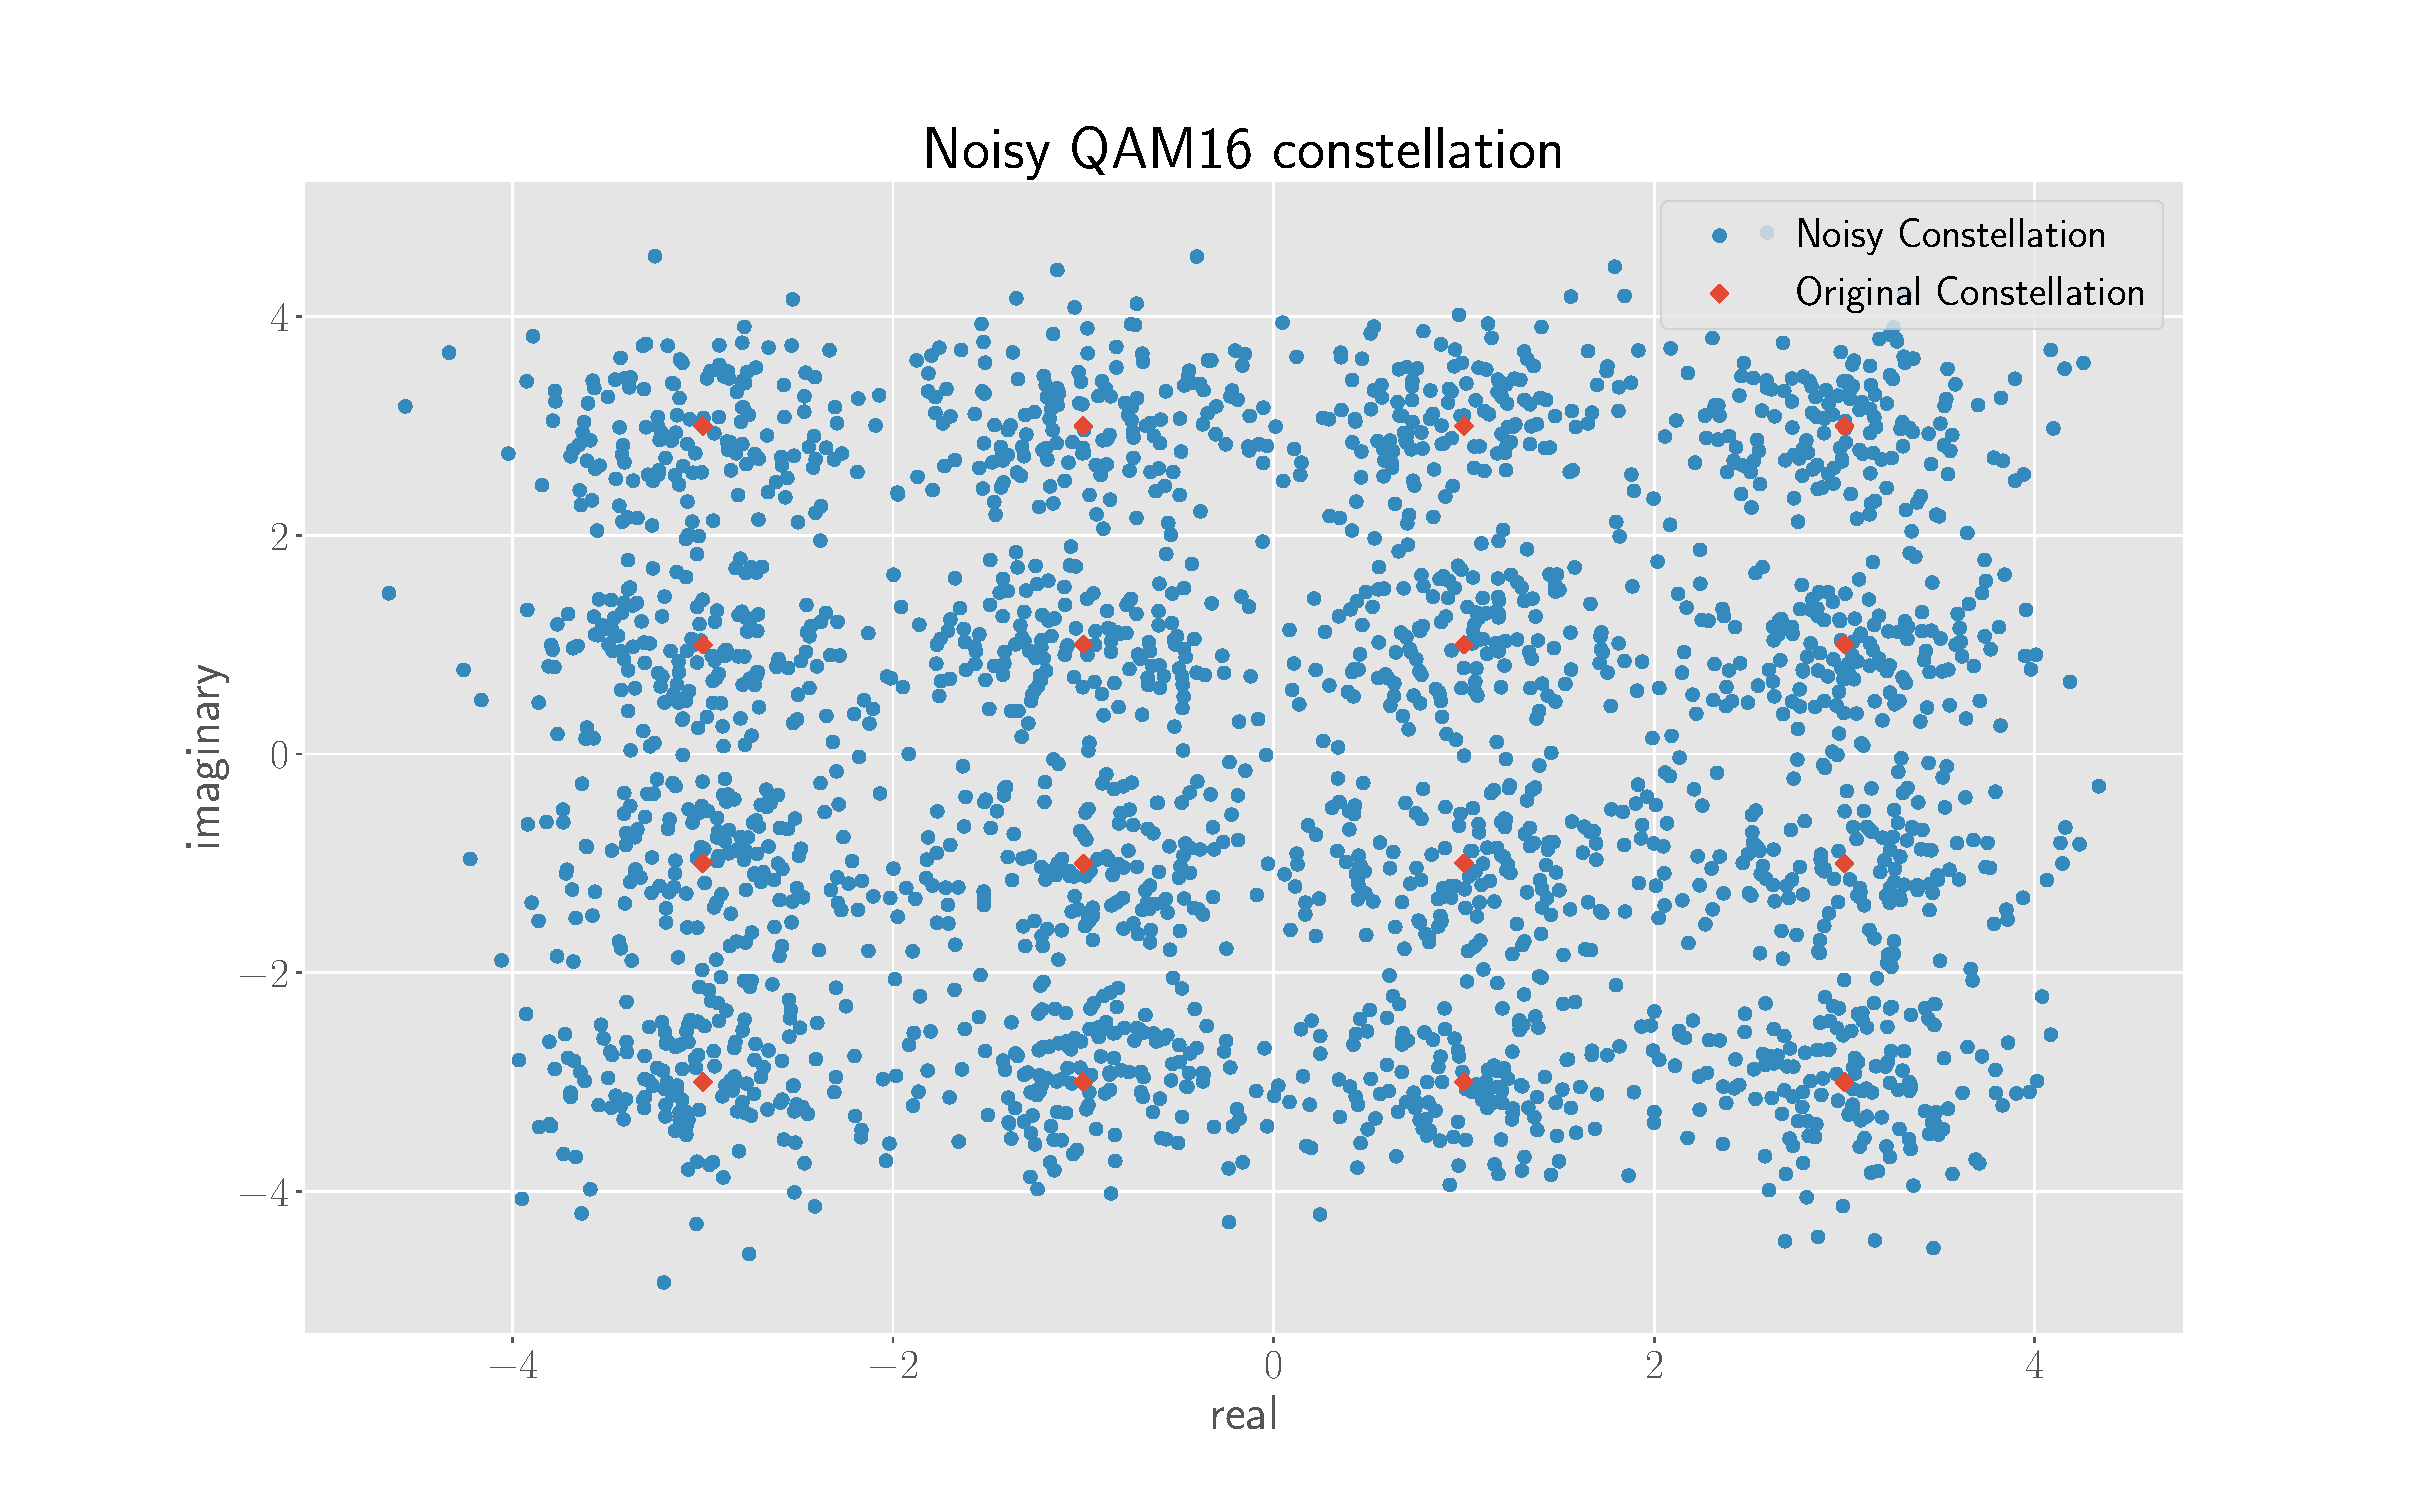
\includegraphics[width=0.763\textwidth]{graphics/constellation.pdf}
  \caption{Noisy constellation used as test data.}\label{fig:noisy_constellation}
\end{figure}


\subsection{Incoherent Integration}

For the incoherent integration, a sinusoidal signal with a frequency of $100\,\si{\hertz}$ was multiplied with a gaussian with standard deviation of $0.01\,\si{\second}$ to create a gaussian-shape spectrum centered around $100\,\si{\hertz}$. The center frequency of each realization was additionally superimposed by random jitter. The signal can be seen in figures \ref{fig:nci_signal}. Figure \ref{fig:nci_signal_spec} shows the realization spectra.

\begin{figure}
    \centering
    \begin{minipage}{0.5\textwidth}
        \centering
        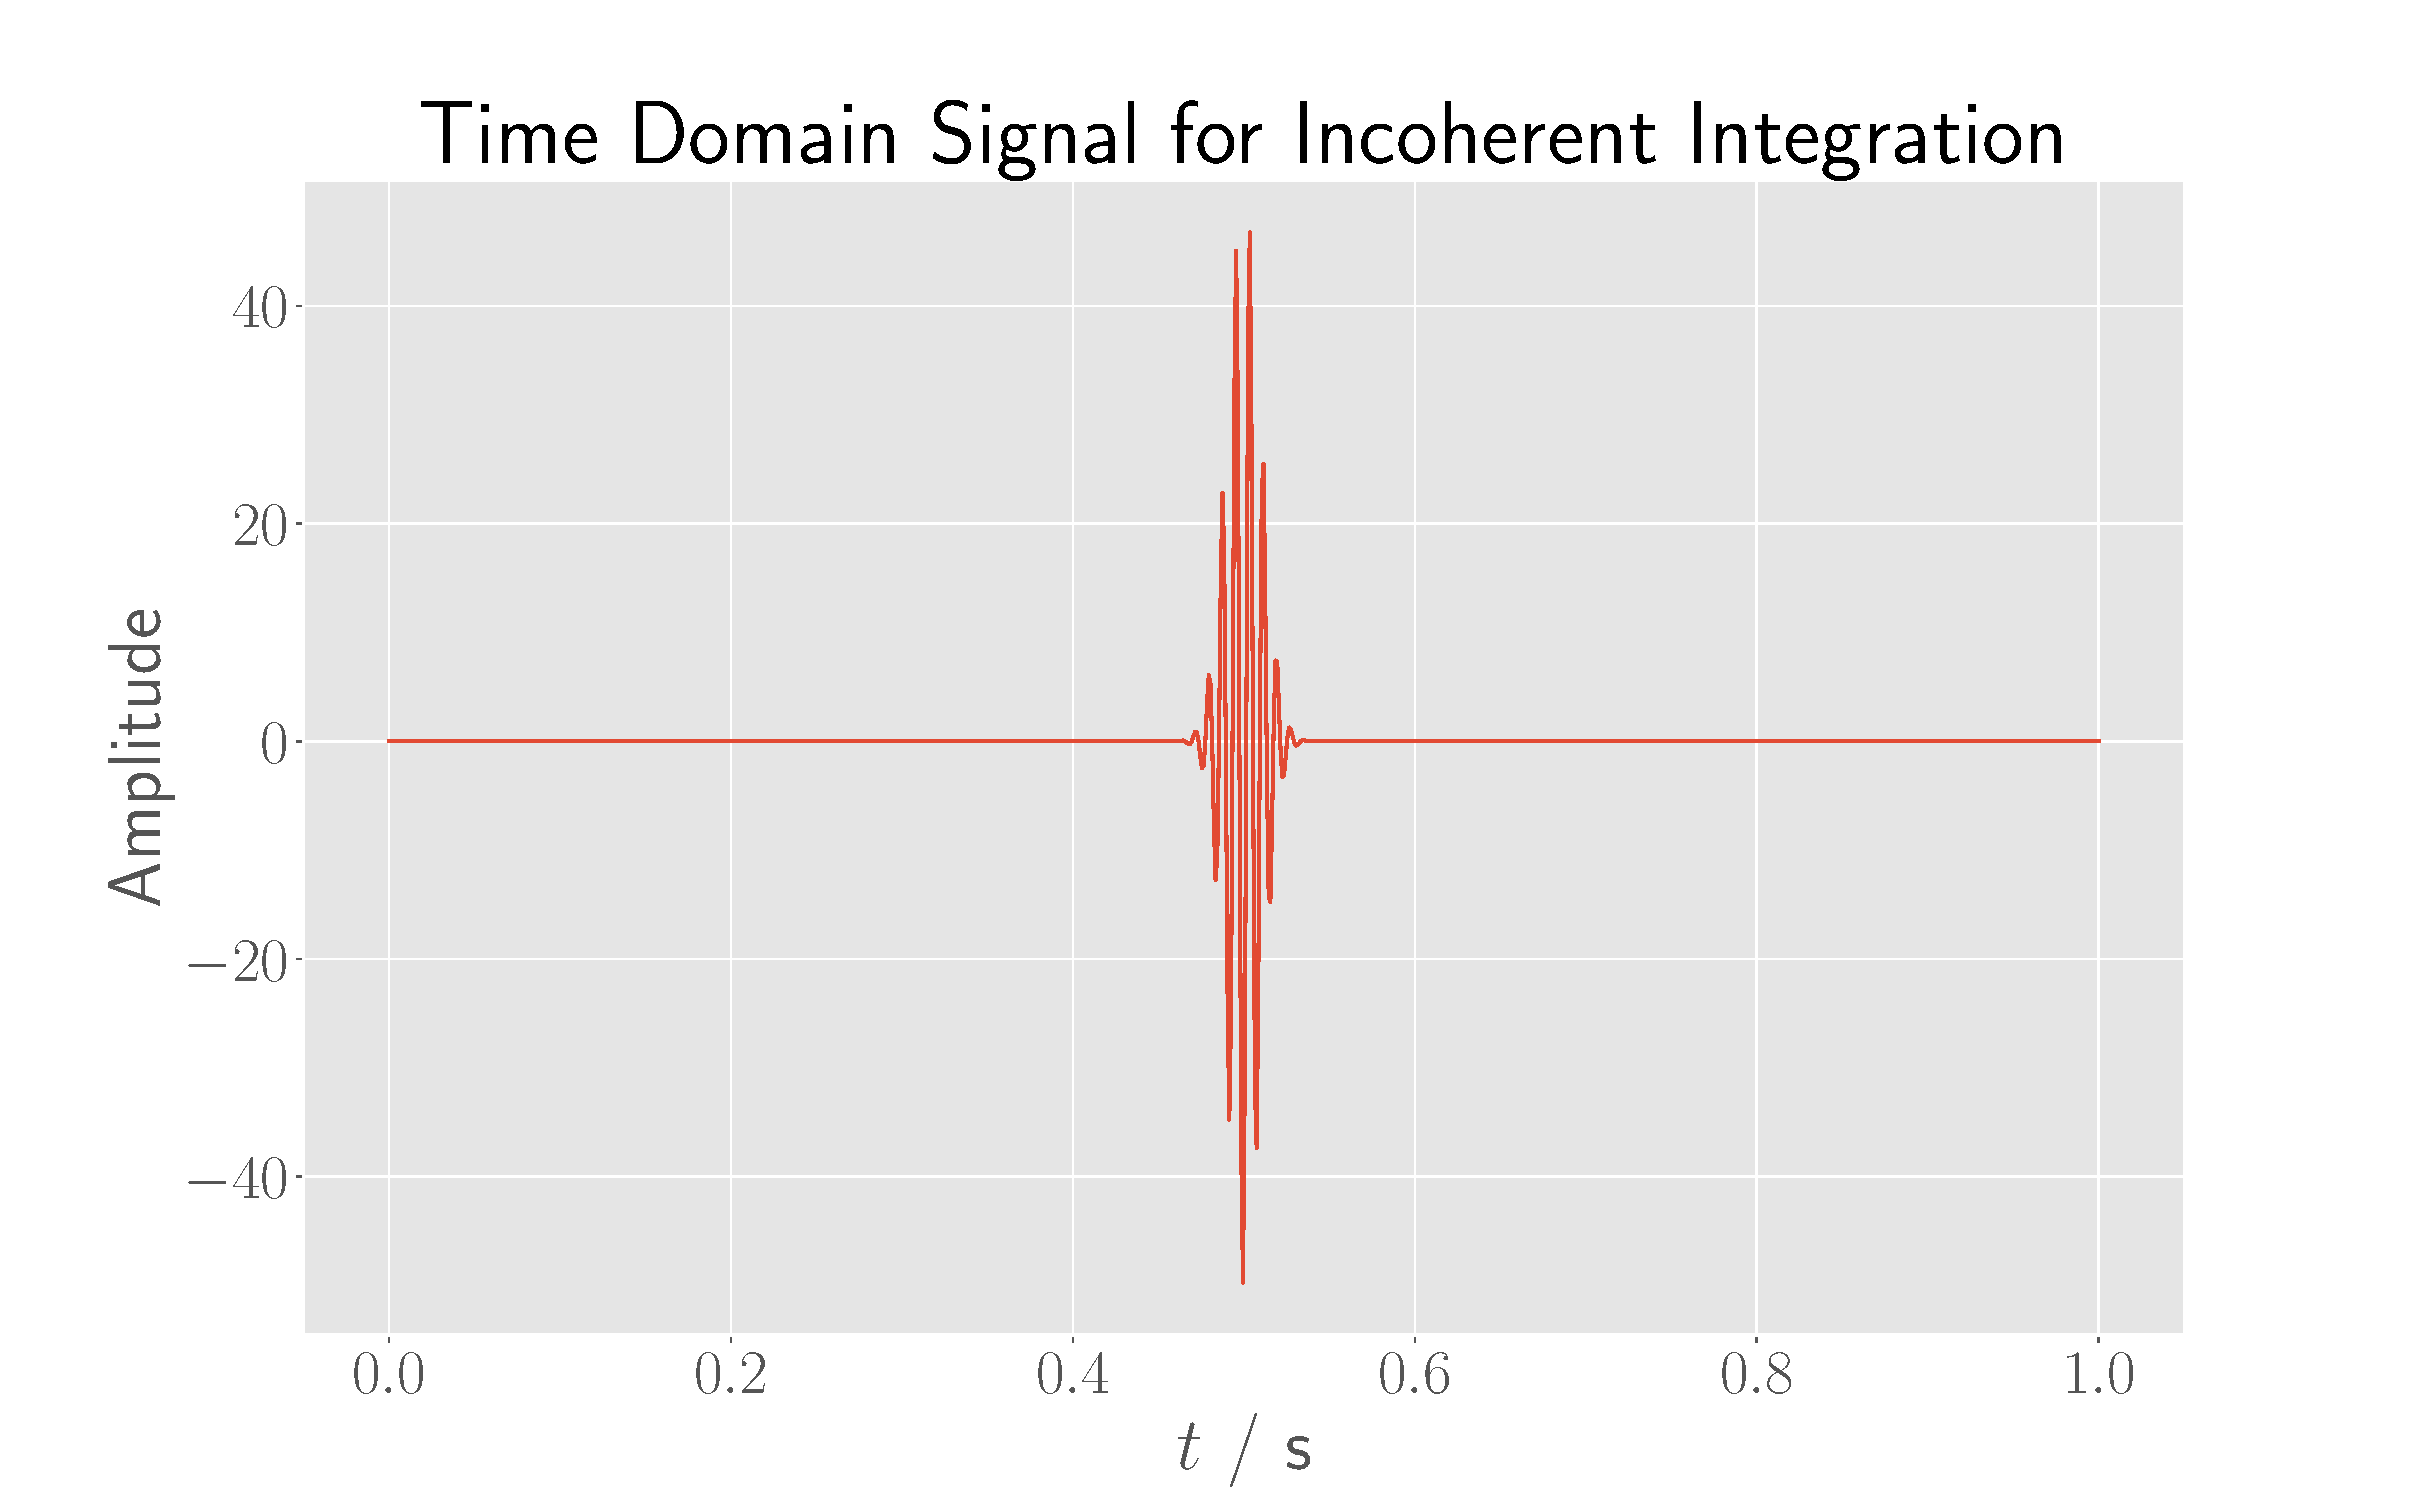
\includegraphics[width=1\textwidth]{graphics/nci_time.pdf} % first figure itself
        \caption{Time domain of NCI test signal (1 realization).}\label{fig:nci_signal}
    \end{minipage}\hfill
    \begin{minipage}{0.5\textwidth}
        \centering
        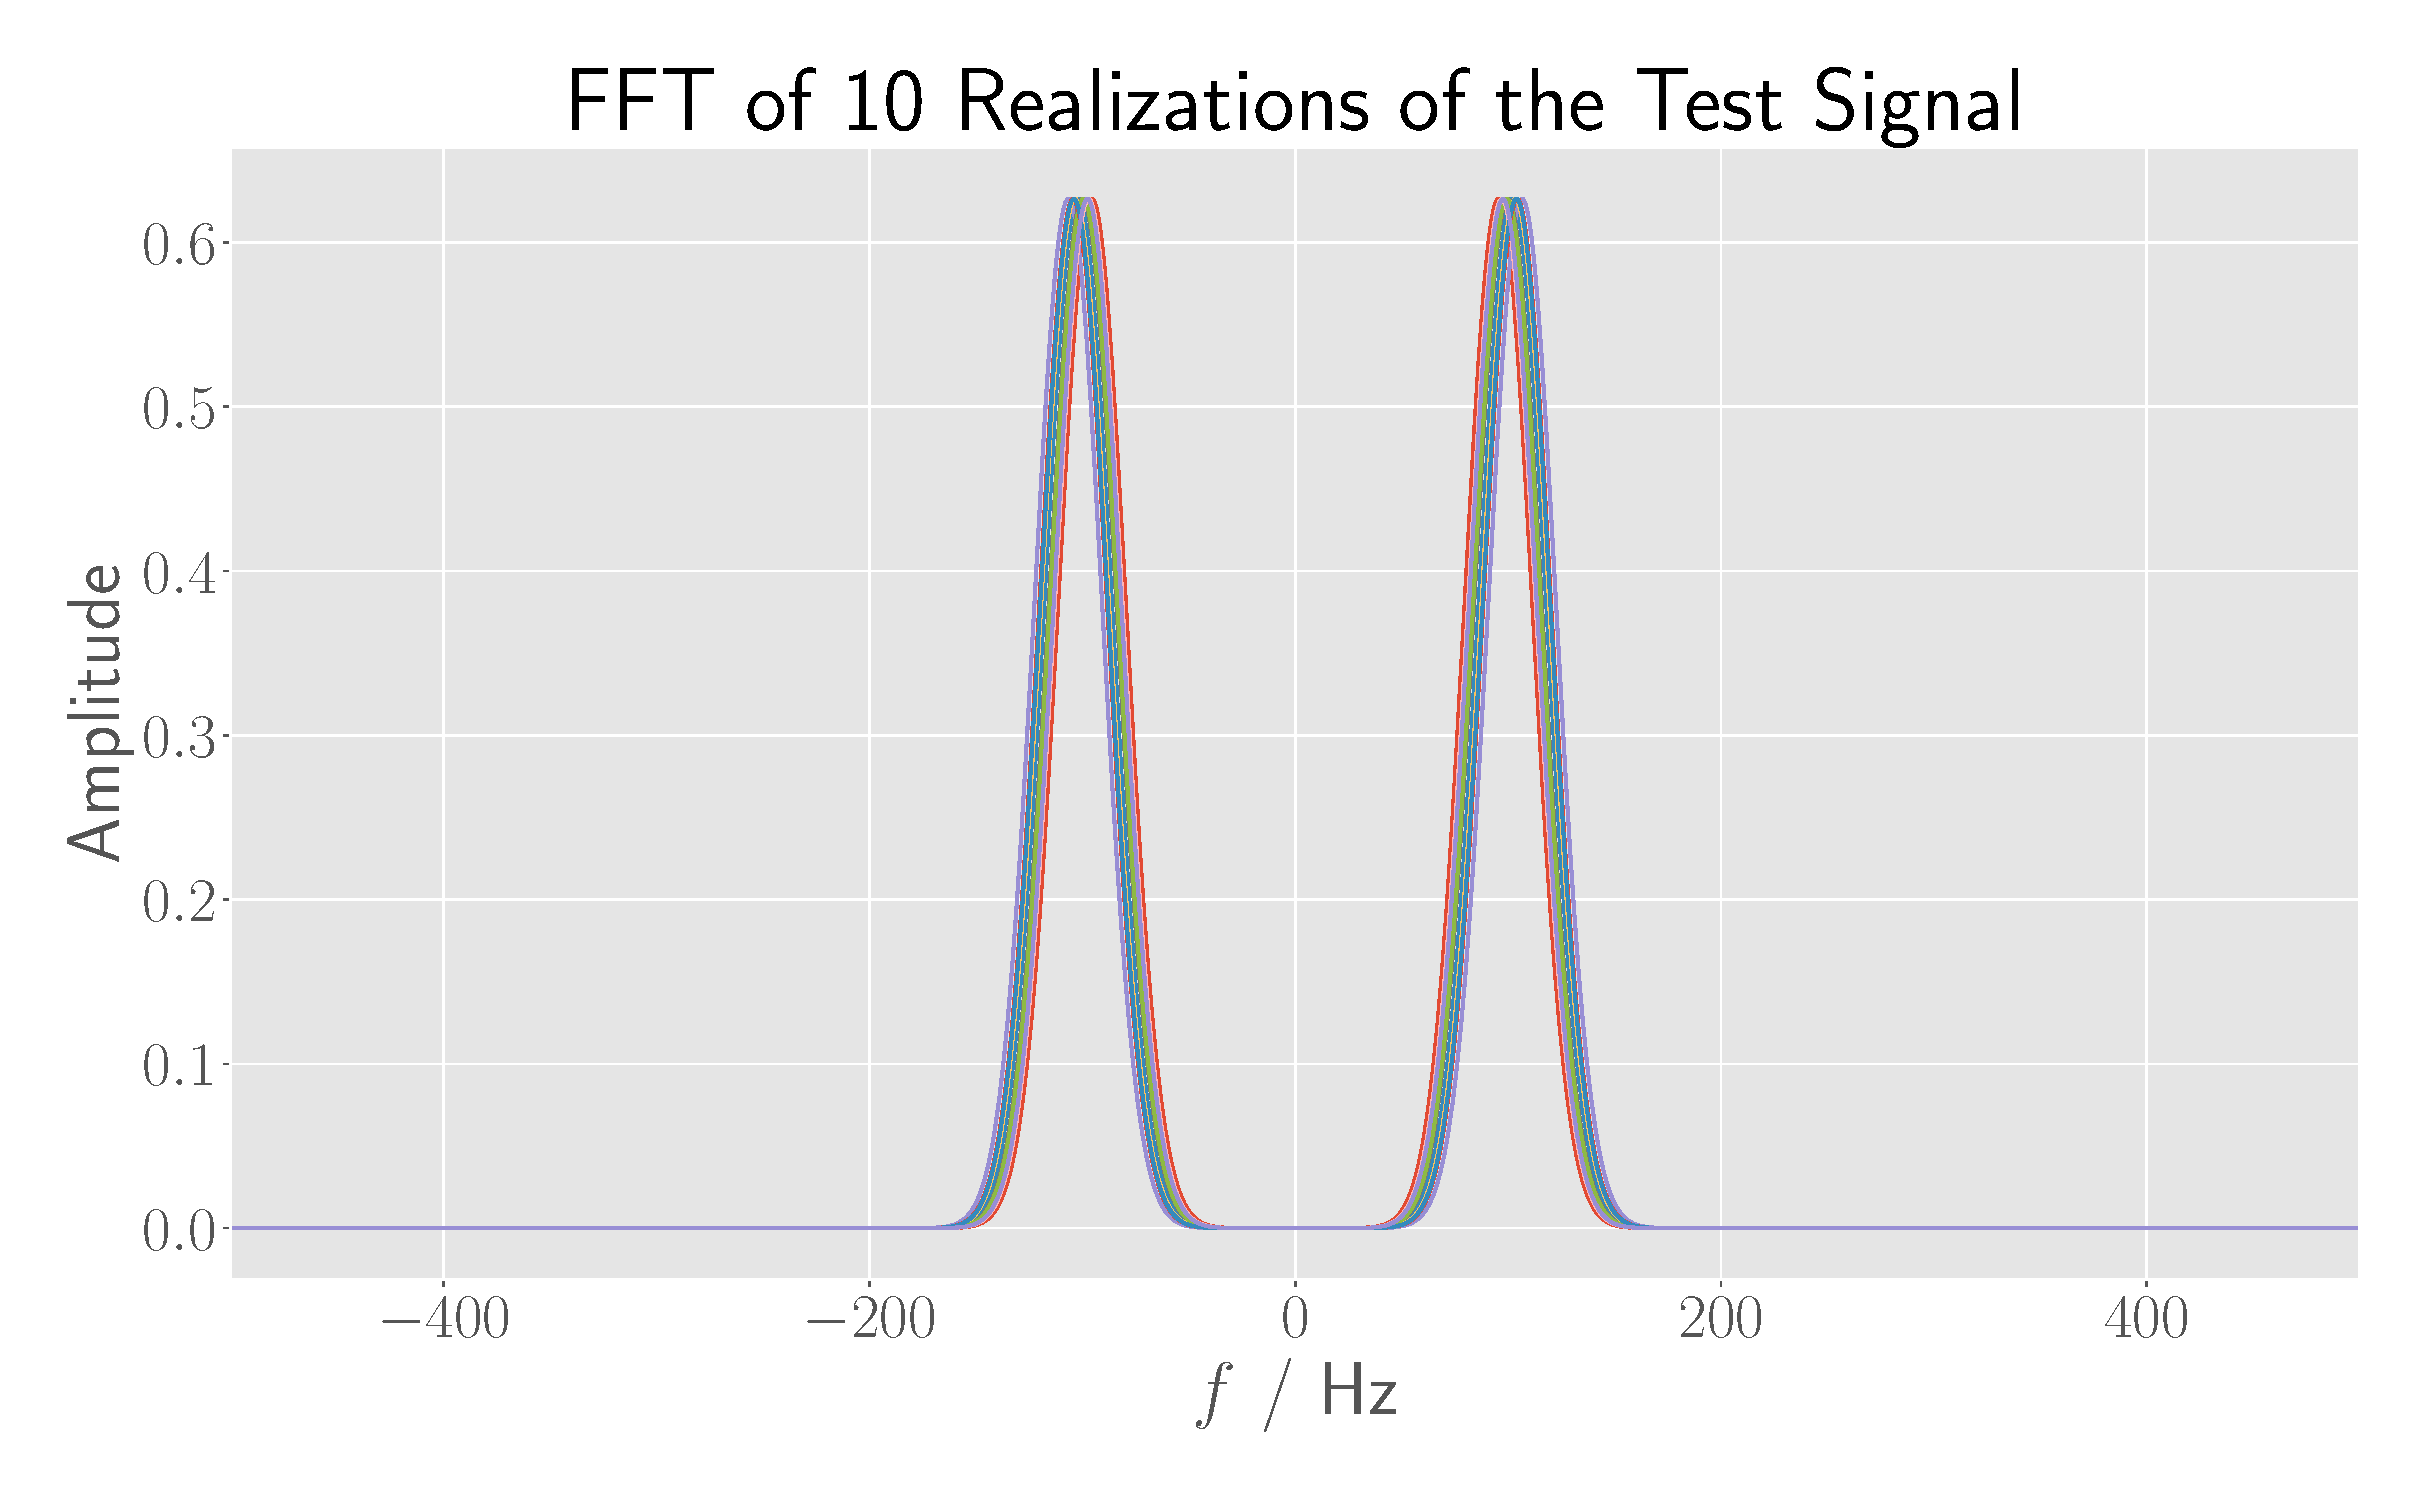
\includegraphics[width=1\textwidth]{graphics/nci_spec.pdf} % second figure itself
        \caption{FFTs of NCI test signals.}\label{fig:nci_signal_spec}
    \end{minipage}
\end{figure}

\subsection{Signal-To-Noise-Ratio}

For the coherent integration, the mean of the squared differences of each noisy sample towards their actual constellation points (the signal without the added noise) was calculated to obtain a measure of noise variance (power, $\sigma^{2}$). The square of the symbol distance ($1\,\si{\volt\squared}$) is then divided by this variance to get the SNR.\\

For incoherent integration, the definition of an SNR is more complicated. \cite{richards_pdf} Here, the SNR was approximated by taking the peak value of the averaged spectrum and dividing it by the noise power (standard deviation squared) which was taken from the first tenth of the spectrum.


\section{Coherent Integration}
% https://www.radartutorial.eu/10.processing/Pulse%20Integration.en.html
% https://www.radartutorial.eu/11.coherent/co05.en.html

With coherent integration, both the real and imaginary parts of a received signal are taken into account (averaged), thereby retaining the phase information. \cite{hysell_radar}\cite{richards_pdf}\\

The integration period (window / sample size) should not be greater than the time that the signal is stable. Otherwise, samples from a different state (amplitude, phase) will be included in the averaging process, which results in a detrimental effect. This can be seen for the $CI=100$ case in both the constellation diagram (figure \ref{fig:ci_const} and the plot of the real part (figure \ref{fig:ci_real}). Since there are $50$ samples per symbol in this case, $CI=100$ leads to two independent symbols being averaged together.\\

\begin{figure}
    \centering
    \begin{minipage}{0.5\textwidth}
        \centering
        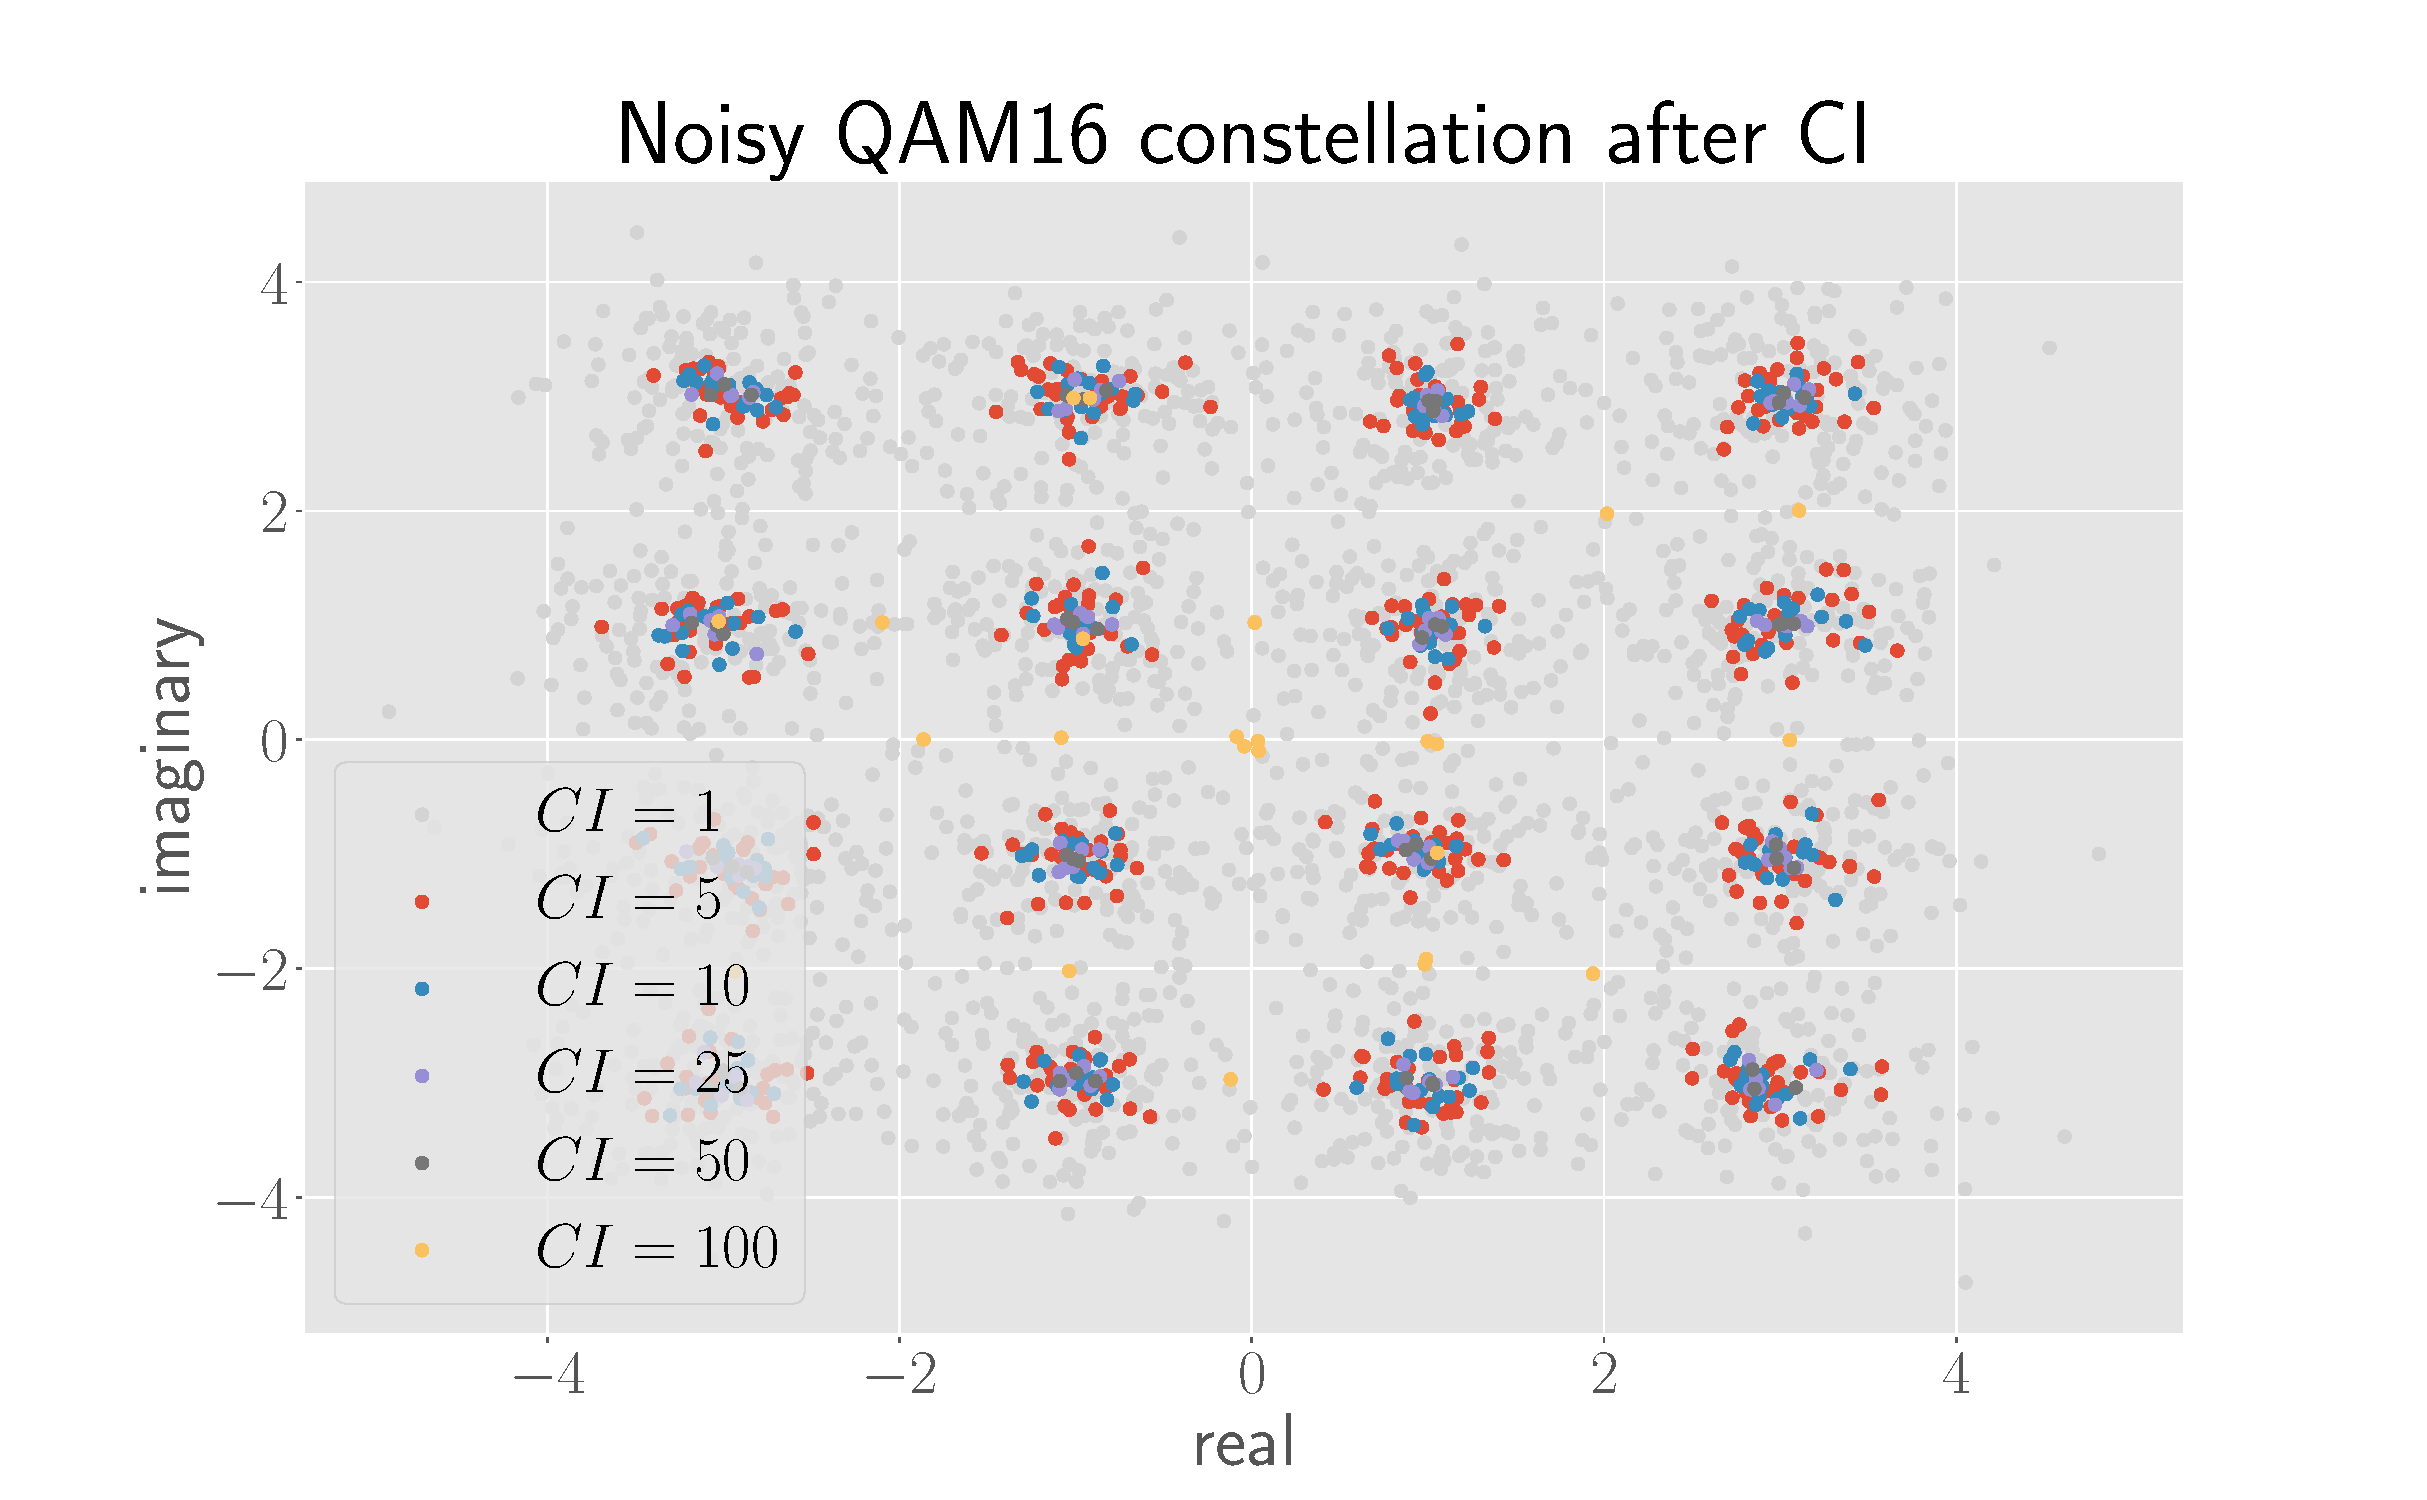
\includegraphics[width=1\textwidth]{graphics/ci_constellation.pdf} % first figure itself
        \caption{Constellation after coherent integration}\label{fig:ci_const}
    \end{minipage}\hfill
    \begin{minipage}{0.5\textwidth}
        \centering
        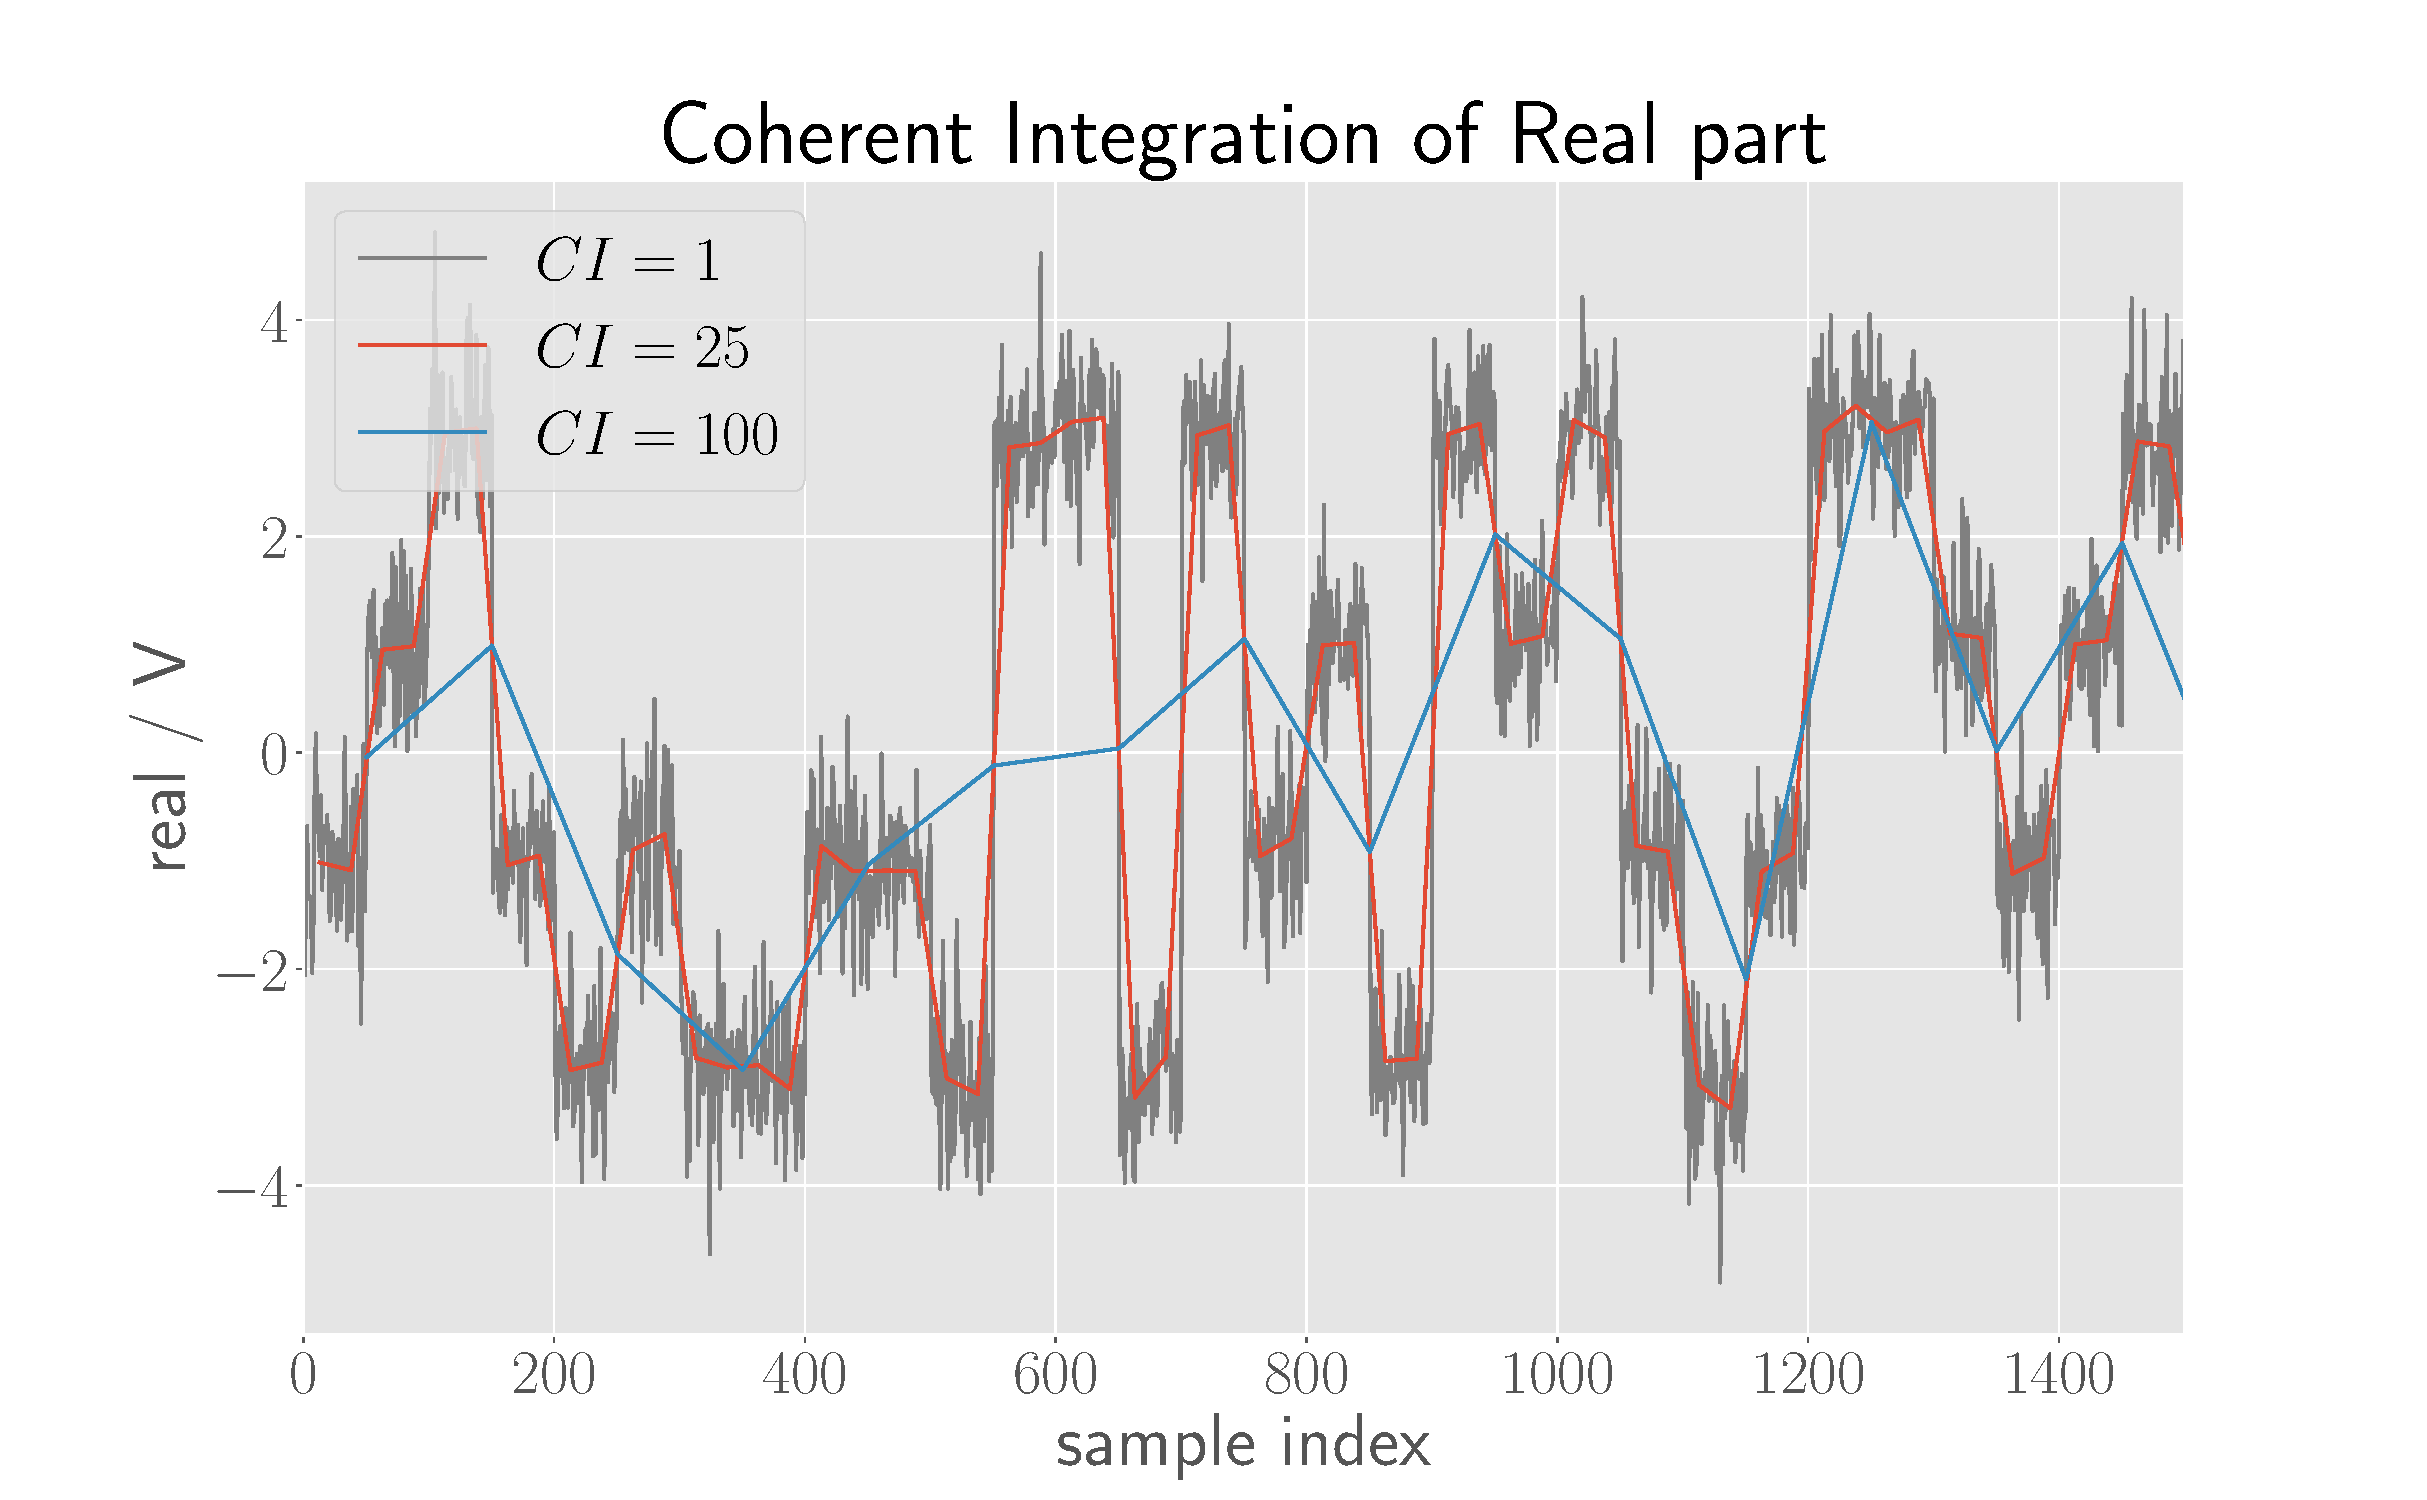
\includegraphics[width=1\textwidth]{graphics/ci_real.pdf} % second figure itself
        \caption{Real part after coherent integration.}\label{fig:ci_real}
    \end{minipage}
\end{figure}

As for the SNR, the noise power rises with $N$ but the signal power rises with $N^{2}$ resulting in an SNR increase which is proportional to the number of integrations. \cite{richards_pdf} Figure \ref{fig:snr_coh} confirms this linear relationship. In figure \ref{fig:snr_coh}, the value at $CI = 100$ is misleading, though. The difference used for the SNR calculation might be high but the actual samples are erroneous which further confirms the fact about the length of the integration period.



\section{Incoherent Integration}
%coh applied to I and Q separately?

For incoherent integration, multiple realizations of the noisy data were translated into the frequency domain. An average of these spectra yields a spectrum (magnitude) which discards the phase information. Like in the coherent case, there is a tradeoff between the SNR gain and the reduced frequency resolution (as one could also take the FFT of the combined realizations). As can be seen in figure \ref{fig:nci_reali}, the noise level is reduced with an increasing number of integrations.\\

\begin{figure}[h]
  \centering
  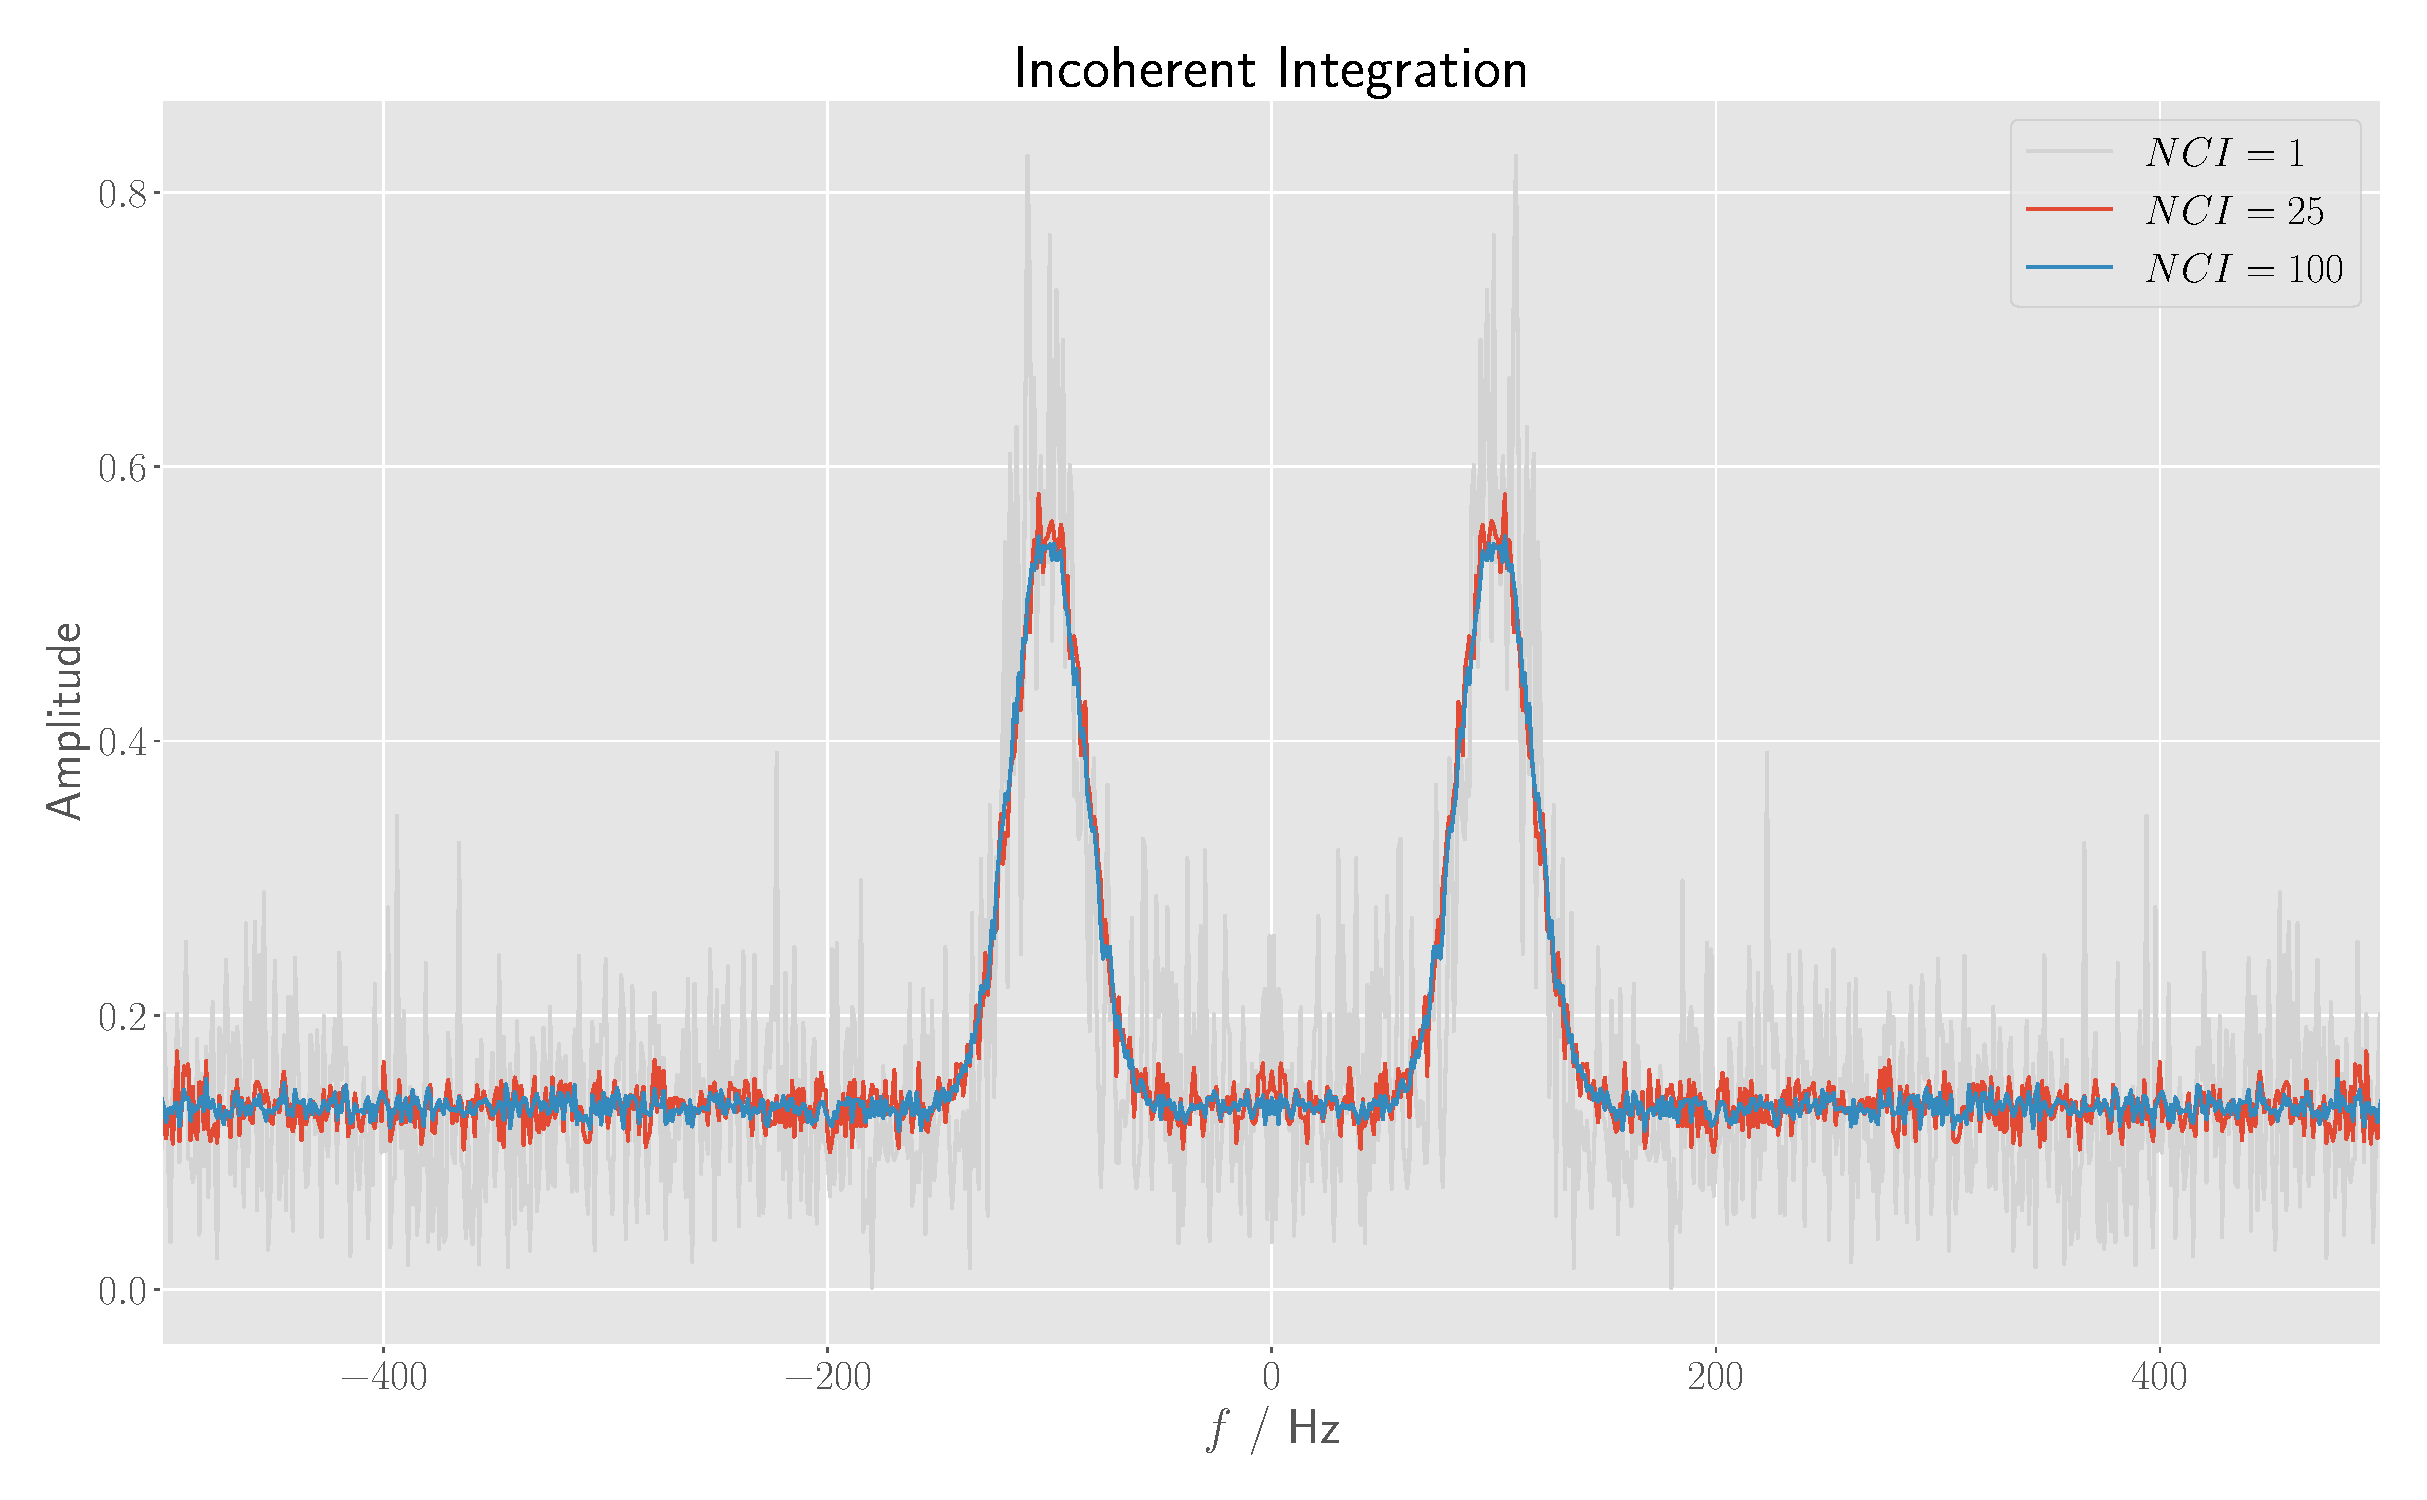
\includegraphics[width=0.763\textwidth]{graphics/rfig.pdf}
  \caption{Resulting spectra after different numbers of incoherent integrations.}\label{fig:nci_reali}
\end{figure}

The result for the SNR can be seen in figure \ref{fig:nci_snr}. Just like in the case of coherent integration, it rises linearly with an increased number of integrations which is as expected \cite{yt_tut}.


\begin{figure}
    \centering
    \begin{minipage}{0.5\textwidth}
        \centering
        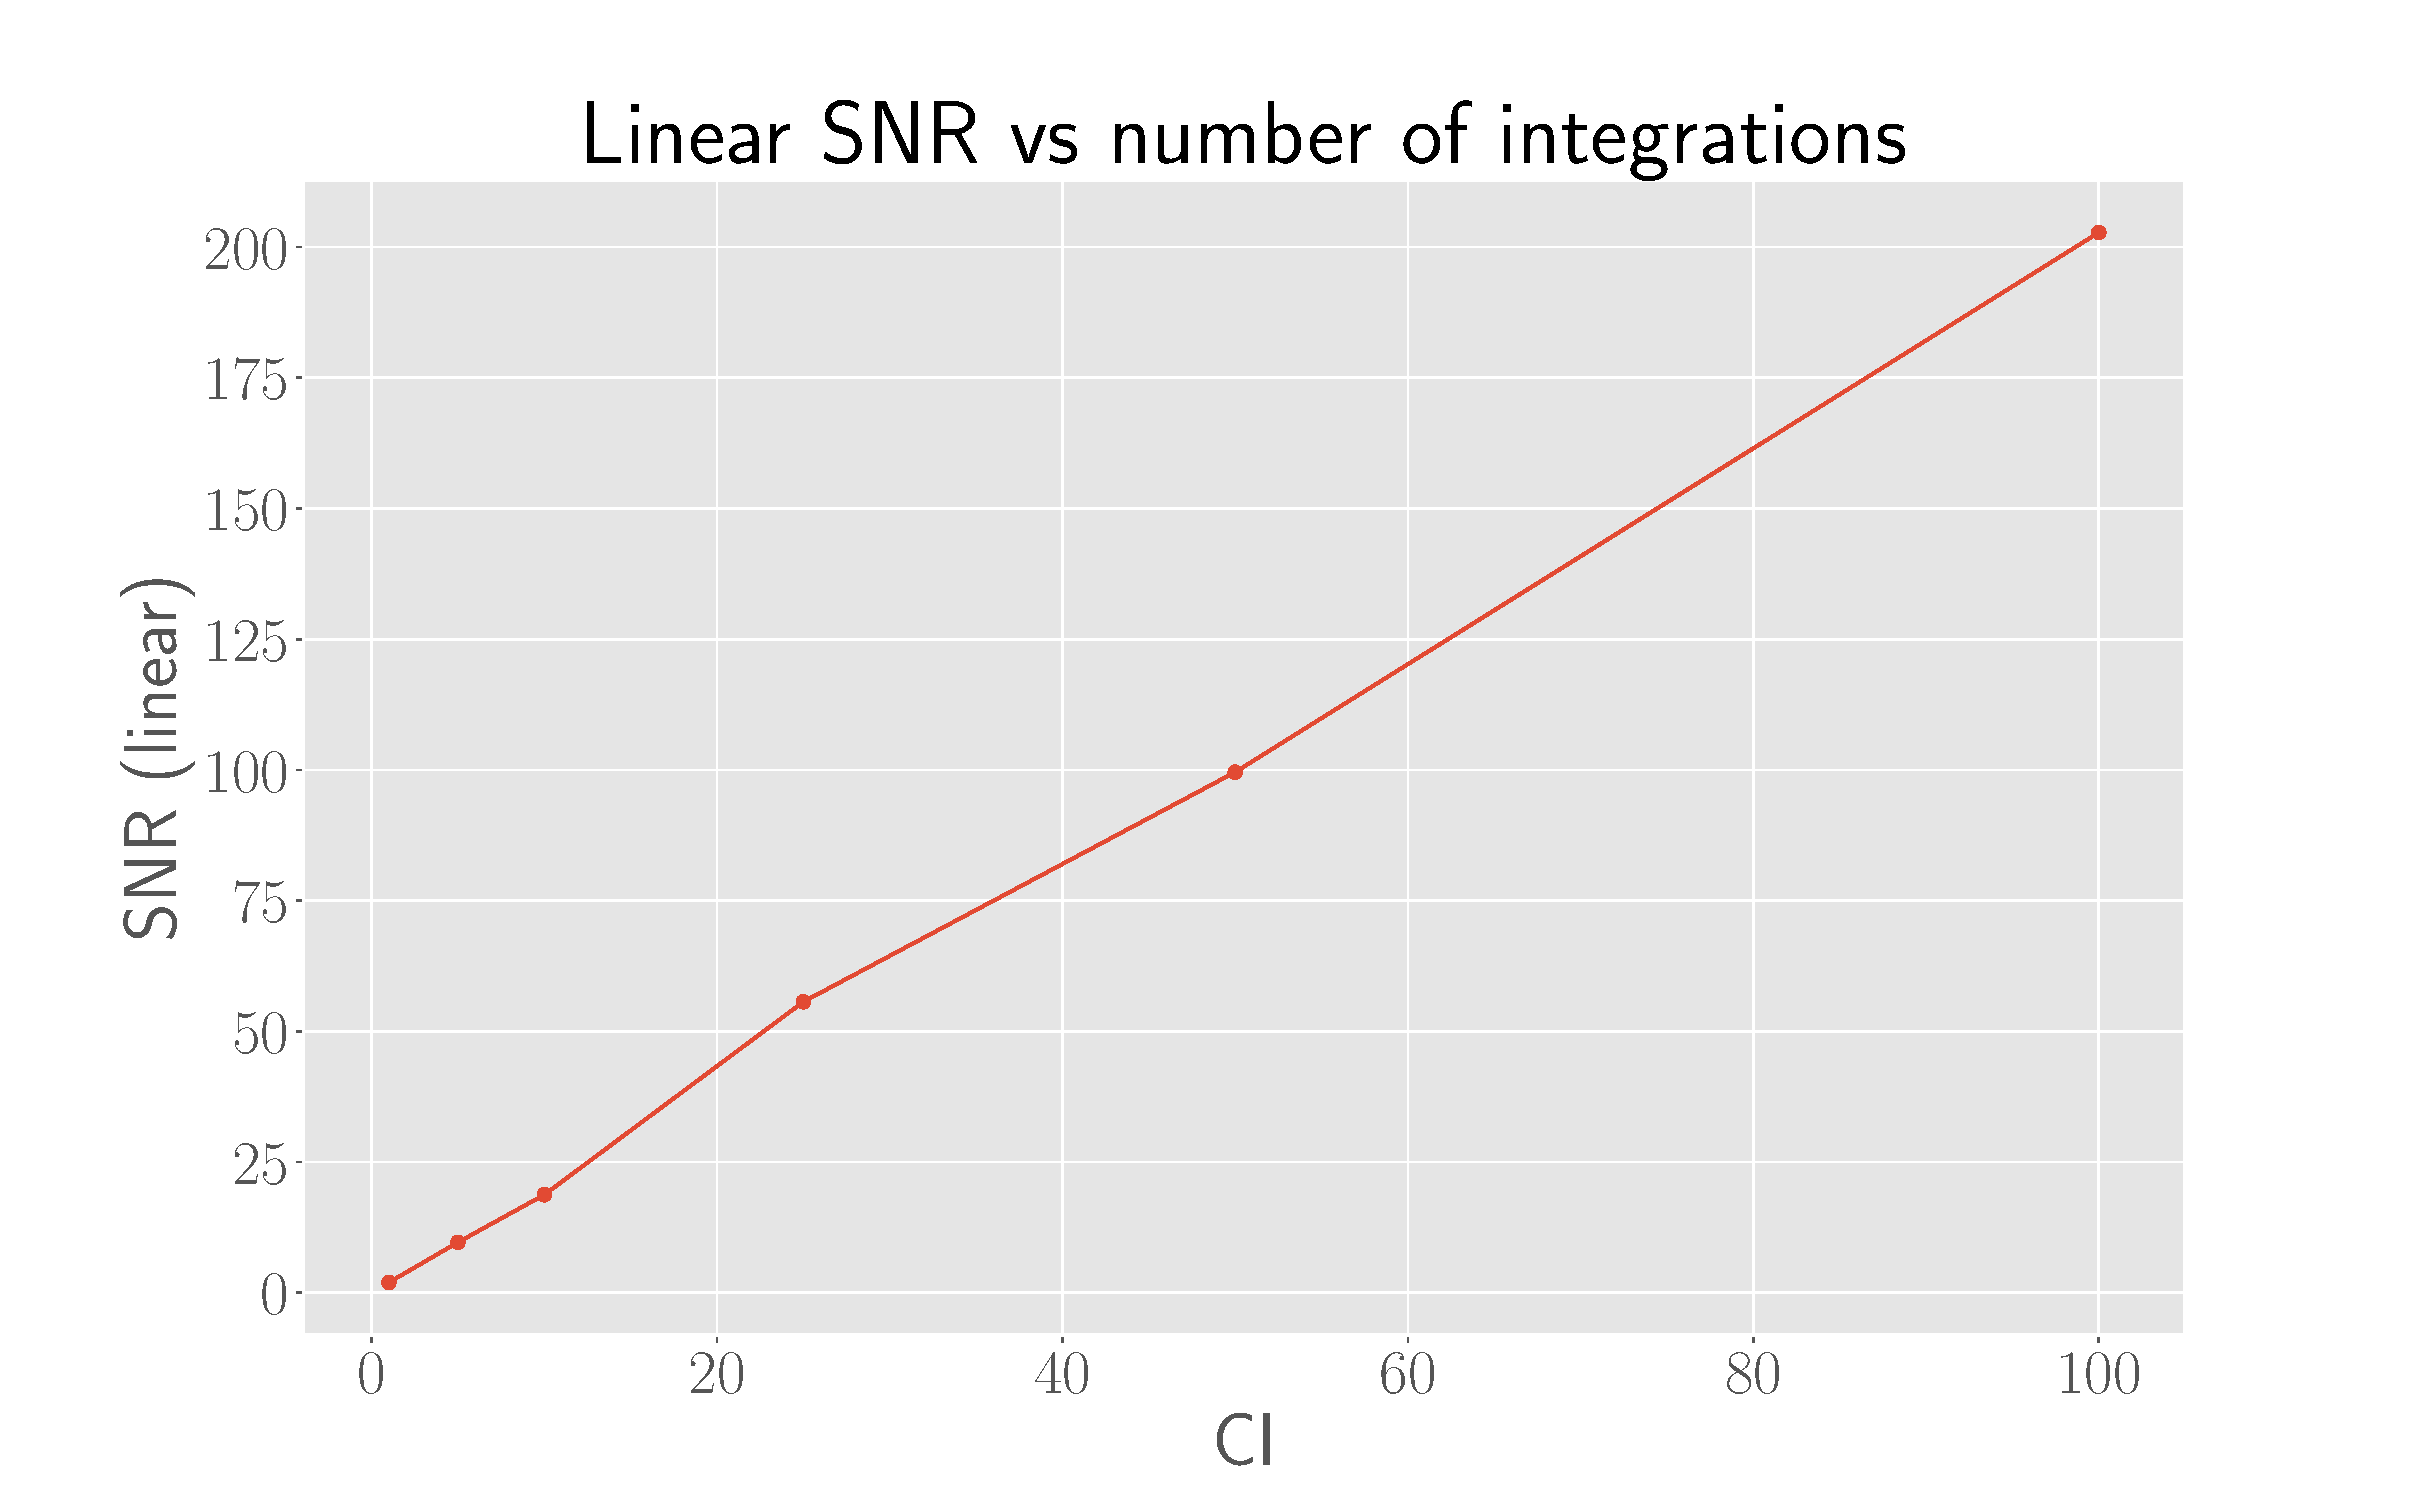
\includegraphics[width=\textwidth]{graphics/ci_snr.pdf}
        \caption{SNR estimate vs number of CIs.}\label{fig:snr_coh}
    \end{minipage}\hfill
    \begin{minipage}{0.5\textwidth}
        \centering
        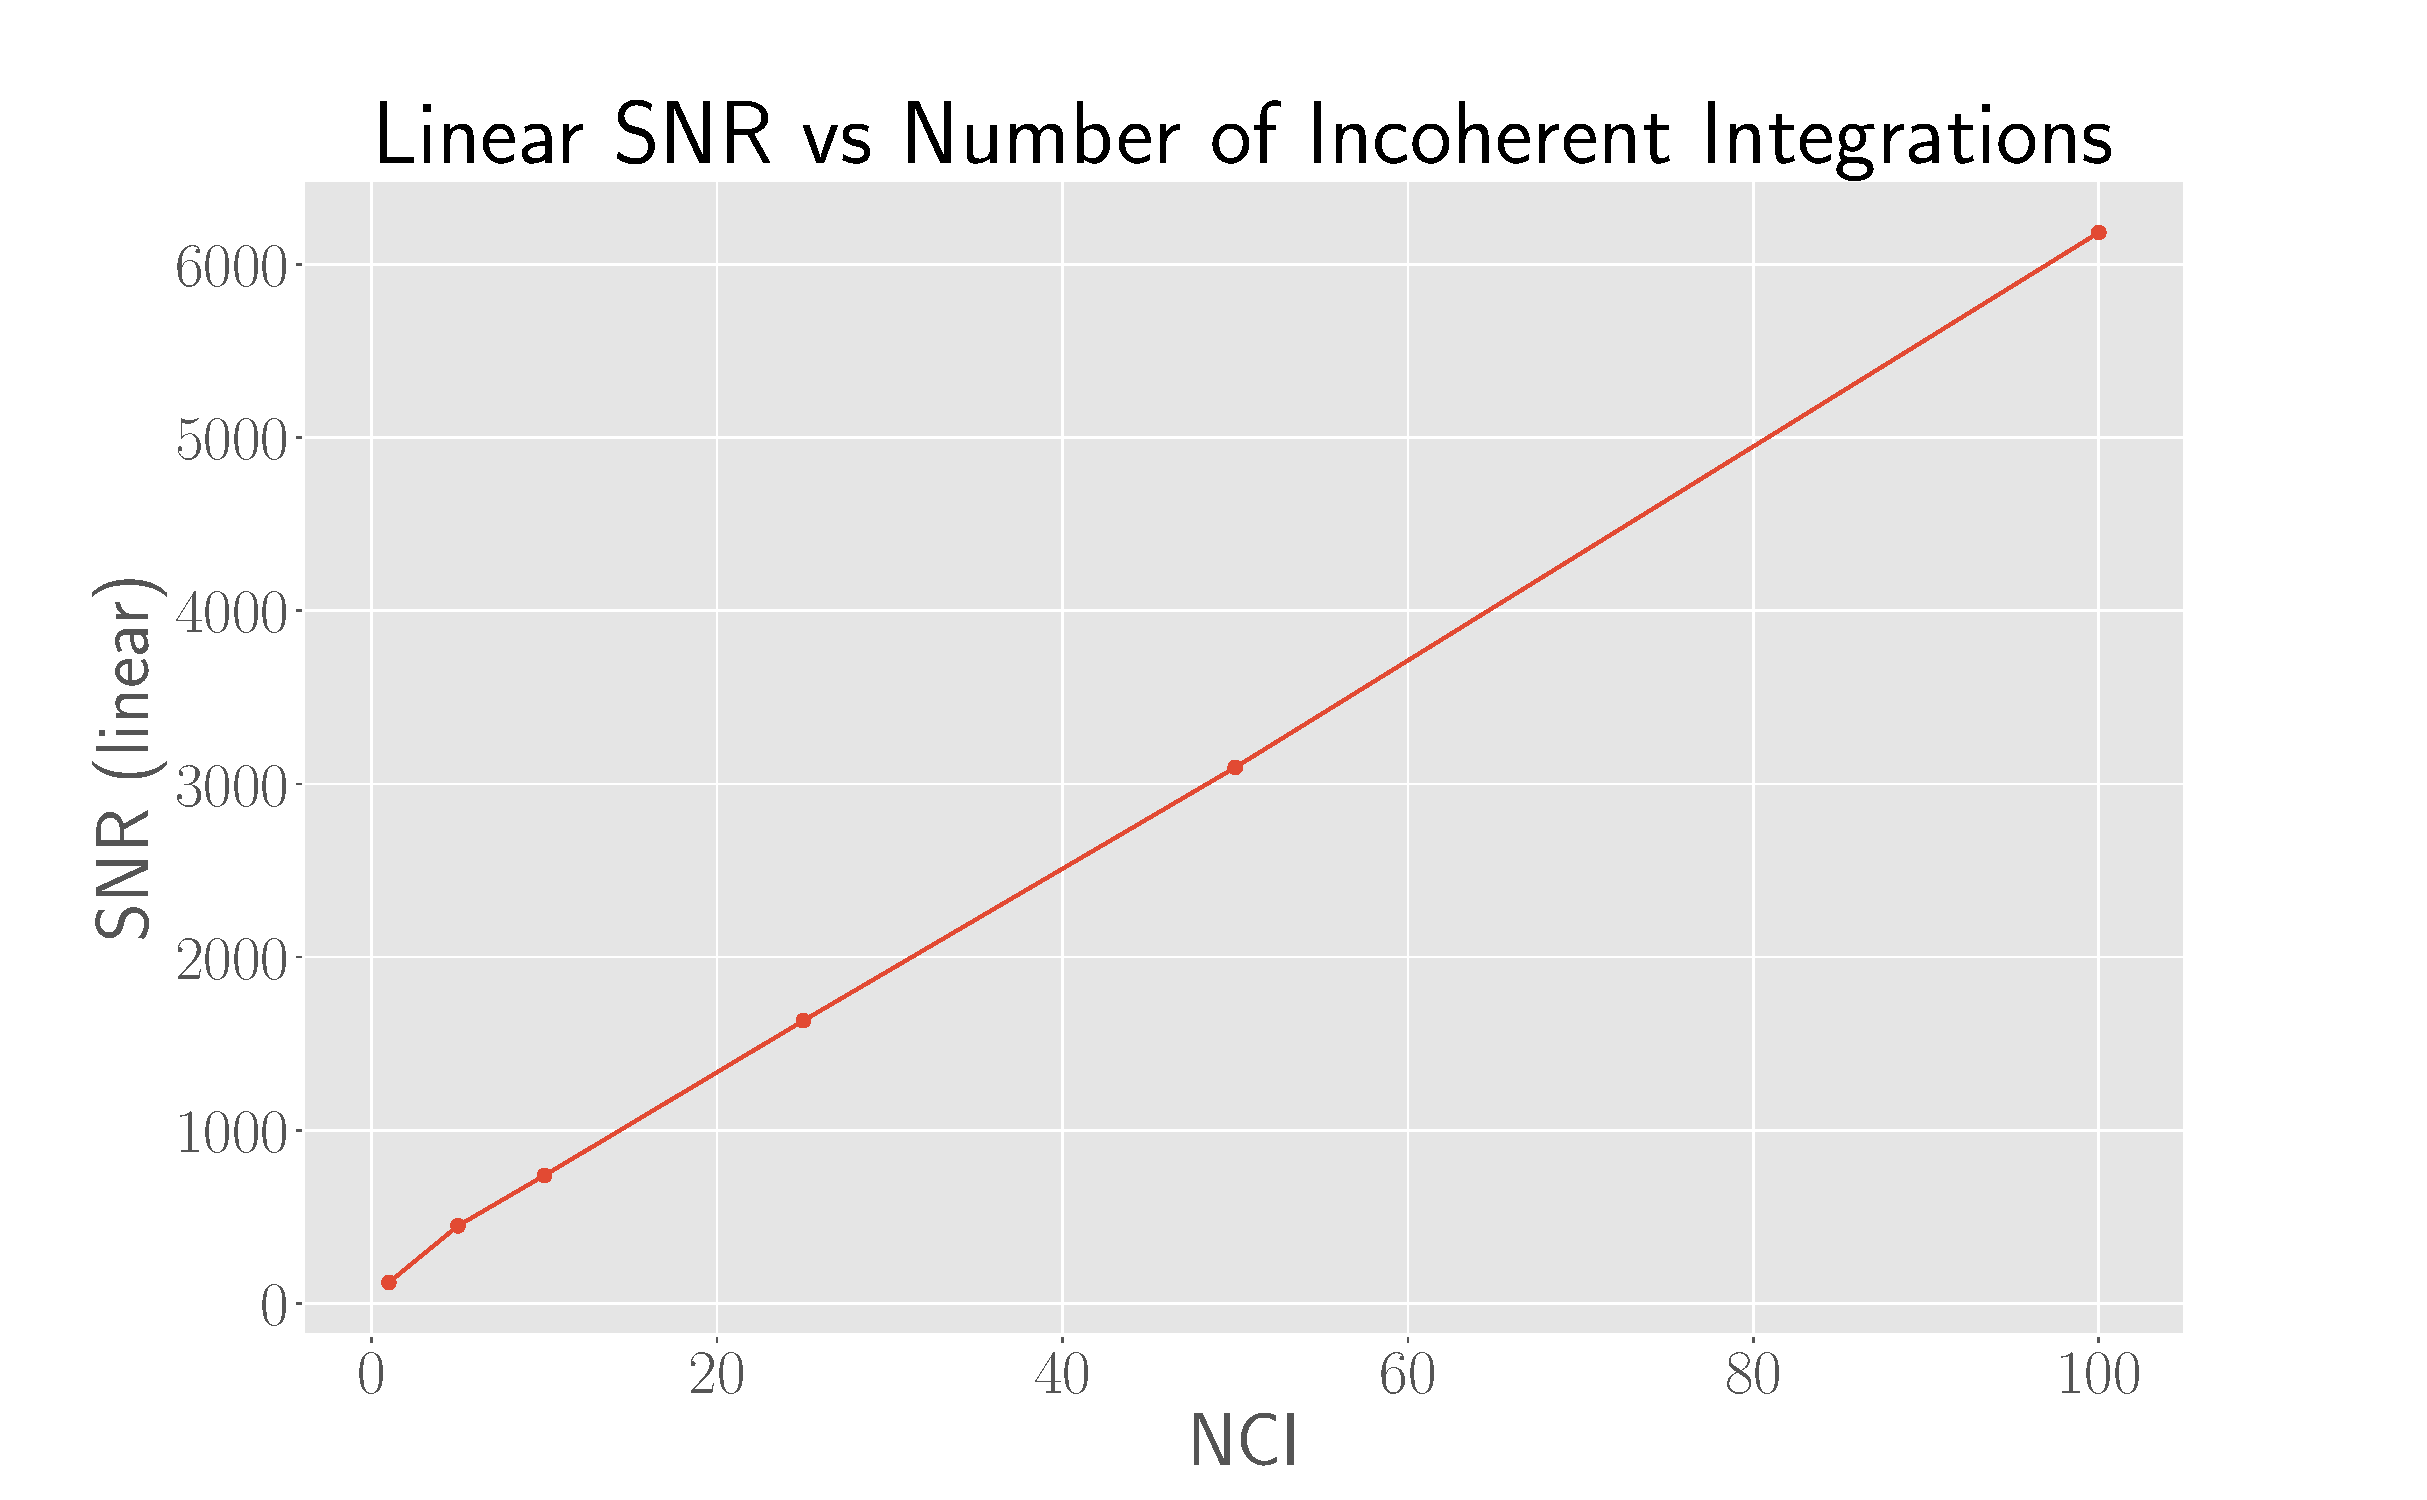
\includegraphics[width=\textwidth]{graphics/nci_snr.pdf}
        \caption{SNR estimate vs number of NCIs.}\label{fig:nci_snr}
    \end{minipage}
\end{figure}


\section{Conclusions}
Coherent and incoherent integrations have been shortly investigated. Coherent integration acts on the complex valued signals and provides a linear SNR gain with increasing numbers of integrations which might be useful in situations where low signal powers are measured or noise is great. The incoherent integration method is simpler and also scales the SNR linearly with the number of integrations. It may be used in cases when the phase information is not needed.


% ------------------------------------------------------------------------------

\printbibheading
\begin{refsection}[sources.bib]
\nocite{*}
\printbibliography[heading=subbibliography,title={Literature}]
\end{refsection}

\begin{refsection}[software.bib]
\nocite{*}
\printbibliography[heading=subbibliography,title={Software Used}]
\end{refsection}

\pagebreak
\appendix
\section{Python Code}\label{app:script}

\subsection{Constellation}\label{app:constellation}
\inputminted{python}{./code/constellation.py}

\subsection{Coherent Integration}\label{app:ci}
\inputminted{python}{./code/coherent_integration.py}

\subsection{Incoherent Integration}\label{app:nci}
\inputminted{python}{./code/incoherent_integration.py}

\end{document}
